\chapter{EXPERIMENT 1: AN INVESTIGATION OF LOCAL AMBIGUITY} \label{ch:exp1}

This chapter aims to verify previous agreement attraction findings in Turkish and investigates whether case syncretism is the main culprit of the agreement attraction effects. 

As discussed in Chapter \ref{ch:accounts}, agreement attraction findings were robust in many languages, and one of the languages they were demonstrated in was Turkish \citep{LagoEtAl2019} with sentences like (\ref{ex:LagoItem}). In a speeded acceptability judgment experiment, where they manipulated the verb's and the attractor's number, they used genitive-marked modifiers as distractors to demonstrate agreement attraction effects. They found that participants accepted ungrammatical sentences with plural genitive attractor compared to single ones.  The reason behind using genitive-marked modifiers was that the nouns with the genitive case ending were commonly used for subject marking in Turkish embedded clauses \citep{GokselKerslake2005,Kornfilt:2011}. Even though previous findings from English showed that possessor phrases do not give rise to agreement attraction effects \citep{NicolEtAl:2016}, \citeauthor{LagoEtAl2019} argued that this is due to the difference in the properties of the genitive cases in English and Turkish. Unlike Turkish, the genitive case is not used as a subject marking in English. Since the genitive-marked nouns frequently function as agreement controllers, they hypothesized that these nouns would partially match with cues in ungrammatical sentences and give rise to attraction effects. 

\ea \label{ex:LagoItem}
    \gll {Teknisyen-\{ler/\O\}-in} {e\u{g}itmen-i} ola\u{g}an{\"u}st{\"u} h{\i}zl{\i} ko\c{s}-tu-\{lar/\O\}.\\
    technician-\{\Pl/\Sg\}-\Gen{} instructor-\Poss{} extraordinarily fast run-\Pst-\{\Pl/\Sg\}\\
    \glt `The technician's/technicians' instructor ran\{\Pl/\Sg\} extraordinarily fast.'
\z

In this chapter, we propose an alternative hypothesis where we argue that previous Turkish findings in the literature resulted from local ambiguity in their experimental sentences. In their experiment, they use consonant-final words, marked with the possessive marking. As we have discussed in Chapter \ref{ch:intro}, when the possessive marking is concatenated to a consonant-final word, its surface form is syncretic with the accusative case as in (\ref{ex:syncretism}). 

\ea \label{ex:syncretism}
    \gll teknisyen-in e\u{g}itmen-i\\
    technician-\Gen{} instructor-\Poss{}/\Acc{}\\
    \glt `technicians's instructor'
\z

\section{Local ambiguity in Turkish agreement attraction}

Due to the aforementioned syncretism, the word \emph{e\u{g}itmeni} may be parsed as either instructor-\Poss{} or instructor-\Acc{}. In the possessive parse, the genitive marking on the word \emph{teknisyenin} is considered the genitive-possessive structure's morphological reflex on the word \emph{teknisyen}. On the other hand, when the word \emph{e\u{g}itmeni} is parsed as instructor-\Acc{}, Turkish speakers have to generate a more complex structure where the word \emph{teknisyenin} is the subject of the embedded clause and the word \emph{e\u{g}itmeni} is the object of the same embedded clause. Sentences (\ref{ex:accParse_lago}) and (\ref{ex:possParse_lago}) exemplify these possible parses. The CP structures are shown with a square brackets. The relative probability of encountering an accusative marking rather than possessive marking also supports the idea of two different interpretations. We calculated the relative likelihood of having an accusative marked noun than a possessive marked noun following genitive marking. Data from some of the annotated treebanks from Universal Dependencies v2.9 \citep{TurkEtAl2021,KuzgunEtAl2020,TurkEtAl2019b,SulubacakEtAl2016} showed that the relative probability of encountering accusative marking after the genitive-marked noun is 0.21.

\ea \label{ex:possibleParses}
    \ea \label{ex:possParse_lago} {Possessive Interpretation}\\*
        \gll [\textsubscript{\it \textsc{cp}}Teknisyen-in e\u{g}itmen-i ko\c{s}-tu.]\\
        \phantom{\normalsize{[\textsubscript{\it \textsc{cp}}}}technician-\Gen{} instructor-\Poss{}[\Nom{}] run-\Pst{}\phantom{]}\\
        \glt `The technician's instructor ran.'
    \ex \label{ex:accParse_lago} {Accusative Interpretation}\\*
        \gll [\textsubscript{\it \textsc{cp}}[\textsubscript{\it \textsc{cp}}Teknisyen-in e\u{g}itmen-i kov-du\u{g}-un-u] g\"{o}r-d\"{u}-m.]\\
        \phantom{\normalsize{[\textsubscript{\it \textsc{cp}}[\textsubscript{\it \textsc{cp}}}}technician-\Gen{} instructor-\Poss{} fire-\Nmlz-\Poss-\Acc{}\phantom{]} see-\Pst-\Fsg{}\phantom{]}\\
        \glt `I saw the technician firing the instructor.'
    \z
\z

When participants treat the {\emph{-I}} marker as a possessive marking (\ref{ex:possParse_lago}), the whole complex DP is assigned a nominative case, the default subject marker in Turkish in main clauses. When participants entertain the possessive parse, they will not need to reanalyze the sentence and process the sentence without any problem. We argue that participants do not exhibit grammatilicaty illusions on those occasions. 

On the other hand, when the accusative parse (\ref{ex:accParse_lago}) is entertained, we hypothesize that participants start maintaining an alternative structure, which will turn out to be erroneous. Given the experimental items, they will be utilizing this structure until they have seen the matrix verb. On those occasions, they will have a structure in which the genitive marked noun is encoded as subject and the \emph{-I} marked noun as the direct object. Even though a reanalysis may correct the final representation, previous studies have shown that an incorrect analysis may still affect the absolute representation and the parsing process (Patson, Darowski, Moon, \& Ferreira, 2009; Staub, 2007). Thus, we hypothesize that this erroneous parses might be the main reason for the agreement attraction effects observed in \cites{LagoEtAl2019} study.

Moreover, psycholinguistics studies have shown that abstract and overt cases that bear morphosyntactic similarities may interfere with the subject-verb dependency \citep{Slioussar2018,ArnettWagers:2017,LogacevVasishth2012}. Given the attested effects of morphosyntax, case, and the lingering effects of abandoned analyses, we hypothesize that the presence of a local ambiguity may lead to an effect similar to mainstream agreement attraction effects. In contrast, we expect that the effect of plural attractor in ungrammatical sentences should be eliminated when the morphological marking is disambiguated early on.

\section{Experiment 1}

To this end, We conducted a speeded acceptability judgment experiment with vowel-ending head nouns. As we discussed in Chapter \ref{ch:intro}, when the possessive and the accusative head follow a vowel-ending noun such as (\emph{y\"onetici}) instead of a consonant-ending noun (\emph{e\u{g}itmen}), their surface form is not syncretic. We provide examples in which a vowel-ending noun is marked with possessive and the accusative case in (\ref{ex:unambSentences}), which are minimally different from sentences in (\ref{ex:possibleParses}). We can see that possessive marking surfaces as {\emph{-sI}} and the accusative as {\emph{-yI}}.

\ea \label{ex:unambSentences}
    \ea \label{ex:unambPossSentence} {Unambiguous Possessive Marking}\\*
        \gll Teknisyen-in y\"onetici-{si} ko\c{s}-tu.\\
        technician-\Gen{} manager-\Poss{}[\Nom{}] run-\Pst{}\\
        \glt `The technician's manager ran.'
    \ex \label{ex:unambAccSentence} {Unambiguous Accusative Marking}\\*
        \gll Teknisyen-in y\"onetici-{yi} kov-du\u{g}-un-u g\"{o}r-d\"{u}-m.\\
        technician-\Gen{} manager-\Acc{} fire-\Nmlz-\Poss-\Acc{} see-\Pst-\Fsg{}\\
        \glt `I saw the technician chasing the manager.'
    \z
\z

We utilized these facts of Turkish and replaced the head nouns in \cites{LagoEtAl2019} items with unambiguous ones. We also modified the rest of the sentence due to plausibility reasons. If the morphosyntactic similarity was a driving factor in Turkish agreement attraction facts, we expected no or substantially reduced difference in acceptability percentages between sentences (\ref{ex:exp1_teasePLPL}) and (\ref{ex:exp1_teaseSGPL}).

\ea \label{ex:exp1MaterialTease}
    \ea[*]{\label{ex:exp1_teasePLPL} {Plural Attractor, Ungrammatical (Plural Verb)}\\*
        \gll {Milyoner-ler-in} {terzi-si} tamamen gereksizce kov-ul-du-lar.\\
        millionaire-\Pl-\Gen{} tailor-\Poss{} completely without\_reason fire-\Pass-\Pst-\Tpl{}\\
        \glt `The millionaires' tailor were fired for no reason at all.'}
    \ex[*]{\label{ex:exp1_teaseSGPL} {Singular Attractor, Ungrammatical (Plural Verb)}\\*
        \gll {Milyoner-in} {terzi-si} tamamen gereksizce kov-ul-du-lar.\\
        millionaire-\Gen{} tailor-\Poss{} completely without\_reason fire-\Pass-\Pst-\Tpl{}\\
        \glt `The millionaire' tailor were fired for no reason at all.'}
    \z
\z

\subsection{Participants}
Our participants (N = 118) were native Turkish speakers and Bo\u{g}azi\c{c}i University undergraduate students. In exchange for attending the experiment, they were given extra credit in one of the pre-determined Linguistics courses. The average age of participants was 20, ranging from 18 to 32. In the experimental process, both the principles of the Declaration of Helsinki and the regulations concerning research ethics at Bo\u{g}azi\c{c}i University were followed without any exception. Our Ethics Committee Approval can be find in Appendix \ref{ap:ethics}. Before the experiment, all participants were asked to provide informed consent. During the experiment, any information regarding their identities was not collected. 

\subsection{Materials}

In our study, we have used 40 sets of sentences like (\ref{ex:exp1items}), where we manipulated both the number of the attractor and the number agreement of the verb (grammatically). The plural markings on the noun and the verb are marked with the suffix \textit{-lAr}. On the other hand, the lack of the suffix \textit{-lAr} on nouns means that they are singular in non-generic environments.\footnote{In generic environments, bare nouns may have kind readings which have been previously shown to increase the magnitude of agreement attraction effects. We avoided generic environments by using an overt past tense morpheme \emph{-DU}.} As for the verbal elements, even though the absence of the suffix \textit{-lAr} does not necessarily indicate singular verbs, we believe that this will not create a problem for us since this paradigm is already shown to be effective in \citeand{LagoEtAl2019}. We used \cites{LagoEtAl2019} items for all of our experimental items as a starting point. We have changed the head noun with a vowel-ending one. We also modified other parts of sentences for plausibility reasons when needed. One item set is given below in (\ref{ex:exp1items}), where the subject phrase is marked with square brackets, and the dependency between the subject head and the matrix verb is signaled using bold-face.

\ea \label{ex:exp1items}
    \ea[*]{{Plural Attractor, Ungrammatical (Plural Verb)} \label{ex:exp1-plpl}\\*
    \gll {Milyoner-ler-in} {terzi-si} tamamen gereksizce kov-ul-du-lar.\\
    millionaire-\Pl-\Gen{} tailor-\Poss{} completely without\_reason fire-\Pass-\Pst-\Tpl{}\\
    \glt `The millionaires' tailor were fired for no reason at all.'}
    \ex[]{{Plural Attractor, Grammatical (Singular Verb)} \label{ex:exp1-plsg} \\*
    \gll {Milyoner-ler-in} {terzi-si} tamamen gereksizce kov-ul-du.\\
    millionaire-\Pl-\Gen{} tailor-\Poss{} completely without\_reason fire-\Pass-\Pst{}\\
    \glt `The millionaires' tailor was fired for no reason at all.'}
    \ex[*]{{Singular Attractor, Ungrammatical (Plural Verb)} \label{ex:exp1-sgpl}\\*
    \gll {Milyoner-in} {terzi-si} tamamen gereksizce kov-ul-du-lar.\\
    millionaire-\Gen[\Sg] tailor-\Poss{} completely without\_reason fire-\Pass-\Pst-\Tpl{}\\
    \glt `The millionaire's tailor were fired for no reason at all.'}
    \ex[]{{Singular Attractor Grammatical (Singular Verb)} \label{ex:exp1-sgsg}\\*
    \gll {Milyoner-in} {terzi-si} tamamen gereksizce kov-ul-du.\\
    millionaire-\Gen[\Sg] tailor-\Poss{} completely without\_reason fire-\Pass-\Pst{}\\
    \glt `The millionaire's tailor was fired for no reason at all.'}
    \z
\z

All experimental sentences followed a pre-determined template: $NP_1(-PL)-GEN{\ }{\ }NP_2-POSS{\ }{\ }Adjunct{\ }{\ }VP-PST(-PL)$. As shown in the template, initial nouns were marked with the genitive and possessive marking, and they formed a complex subject like \textit{milyonerlerin terzisi}, (\textit{the millionaires' tailor}). The genitive-marked NP, the possessor, functioned as the attractor, and the head noun carried an unambiguous possessive case marker. The head noun was always singular, making sentences that contain a verb marked overtly with \textit{-lAr} ungrammatical. Moreover, we have not changed the semantic relationship between the initial NPs. Genitive-possessive structures can be paraphrased using \textit{'s} or \textit{of} in English as in \cites{LagoEtAl2019} study. Adjuncts, pre-verbal adverbials, were 15 characters long on average and consisted of two or three words. Lastly, we followed the distribution of the verb types introduced in the original study: twenty unergatives, eighteen unaccusatives, and two optionally transitive verbs. 


In addition to experimental items, we have used 40 filler items. We hypothesized that some participants might develop a simple response strategy after seeing a certain amount of our experimental items. They may decide on the grammaticality by just looking at the verb number since ungrammatical sentences in our experiment end with a plural marked verb. To prevent this response strategy, we designed our filler items such that plural-agreement-bearing verbs are only seen in grammatical sentences, and singular verbs are only seen in ungrammatical sentences. Half of our filler items (20) ended with a plural-marked verb, while the others ended with a singular verb. Like our experimental items, filler items also started with a complex genitive-possessive noun phrase. However, genitive-possessive noun phrases were the subject of the embedded clause, which functioned as an adverb to the main verb, unlike experimental items where the complex NP is the subject of the main verb. An example set of filler sentences can be found in (\ref{ex:exp1fillers}). All of our experimental and filler items can be found in Appendix \ref{ap:exp1items}.


\ea \label{ex:exp1fillers}
    \ea {Grammatical Filler (Plural Verb)} \label{ex:exp1_gram_filler}\\*
    \gll [Sosyolog-un \"{o}\u{g}renci-si] konu\c{s}-unca tutars{\i}zl{\i}k a\c{c}{\i}\u{g}-a \c{c}{\i}kar-d{\i}-lar.\\ 
    sociolog-\Gen{}  student-\Poss{} speak-\When{} inconsistency  open-\Dat{} deduct-\Pst-\Pl{}\\
    \glt `When the student of the sociologist spoke, they revealed an inconsistency.'
    \ex[*]{{Ungrammatical Filler (Singular Verb)} \label{ex:exp1_ung_filler}\\*
    \gll [Dans\"{o}z-\"{u}n koca-s{\i}] var-{\i}nca kap{\i} sakince a\c{c}-t{\i}. \\
    dancer-\Gen{}  husband-\Poss{} arrive-\When{} door slowly  open-\Pst{}\\
    \glt Intended:`When the husband of the dancer came, the door opened slowly.'}
    \z
\z




\subsection{Procedure}

The experiment was run on Ibex Farm \citep{Drummond2013}, a web-based platform for hosting experiments. Each experimental session was completed in less than 30 minutes. Before the experiments, participants were asked to provide their native language and age. They also were asked to provie a consent form that explained the experimental process and their rights in detail. After the consent, they were presented with the instructions and were given nine practice trials.

The structure of each trial is presented in Figure \ref{fig:trial_infographic}. Participants initially saw a blank screen for 600 ms. The blank screen was followed by the sentence given in word-by-word RSVP fashion. Each word was delivered in 30 pt font size with Times New Roman font and centered on the page. Between every word, participants saw a 100 ms blank screen as well. After the sentence was presented, participants were asked to provide a grammaticality judgment. After every trial, participants are asked to indicate their acceptability judgment. The wording of the question is given in (\ref{ex:exp1_question}). 

\begin{figure}[hbt!]
    \centering
    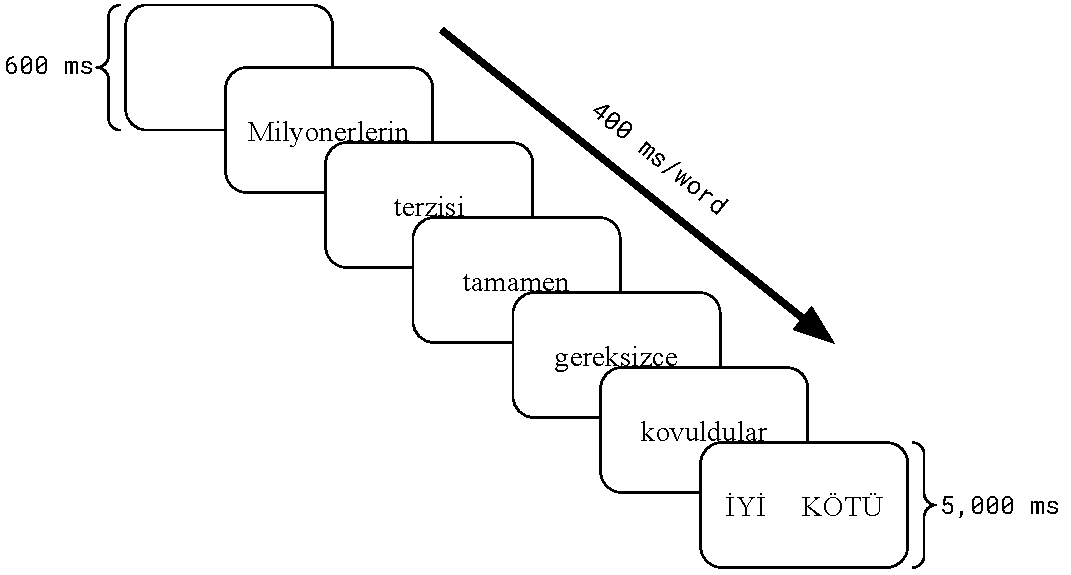
\includegraphics[width=\textwidth]{figure/trial_infographic.pdf}
    \caption{Simplified illustration of RSVP presentation utilized in the experiment}
    \label{fig:trial_infographic}
\end{figure}

\ea \label{ex:exp1_question}
Bu c\"umle kula\u{g}{\i}n{\i}za nas{\i}l geliyor? \\*
`How does this sentence sound to you?'
\z

The possible answers that participants could provide were either \emph{iyi} (good) or \emph{k\"ot\"u} (bad). Participants were asked to press the key P to indicate that a sentence is acceptable/good and Q to indicate that the sentence is unacceptable/bad. Within instructions before the experiments, they were told to provide judgments as soon as possible. If they did not respond within 5,000 ms during the experiment, the trial timed out, and participants were shown the message `\emph{Please respond faster!}' in red font.

Participants saw 40 experimental and 40 filler sentences. Experimental sentences were distributed among four different lists according to a Latin-square design. Every participant saw one version of the experiment with a specific list and one item per condition while seeing all filler items. All items were shuffled, and shuffling was done automatically by the Ibex Farm.

\subsection{Analysis}

Since our central question in this experiment was to test whether or not the existing agreement attraction finding was a product of the local ambiguity in \cites{LagoEtAl2019} experimental sentences due to morphological syncretism, we included \cites{LagoEtAl2019} data to our experimental data. We carried out the Bayesian analysis on our findings in Experiment 1 and on \cites{LagoEtAl2019} findings. As an additional categorical variable, we included the experiment (\citeand{LagoEtAl2019} / Our Experiment) in our Bayesian GLMs.

We excluded some participants using two criteria: (i) their performance in sentences with a singular attractor and (ii) their response time. For all participants, we found their mean percentage of \textit{yes} responses for singular attractor ungrammatical (\ref{ex:exp1-sgpl}) and singular attractor grammatical conditions (\ref{ex:exp1-sgsg}). If the difference between these mean values were below 0.25, that is, they failed to detect ungrammaticality even when there is no attractor to interfere, we excluded all data coming from that participant. In addition, we also excluded trials in which participants were not fast enough to respond ($RT > $ 4999 ms) or participants responded too quickly ($RT < $ 200 ms). After applying these criteria, 11.06\% of the trials from our experiment and 2.38\% of the \cites{LagoEtAl2019} trials. 

We analyzed yes responses with two Bayesian Generalized Linear Models (GLMs). We assumed that responses were distributed following a Bernoulli distribution with a probit link function. We used the R packages brms \citep{R-brms_a,R-brms_b} and rstan \citep{R-rstan} to fit Bayesian hierarchical models \citep[e.g.,][]{GelmanHill:2007, NicenboimVasishth:2016}. We analyzed only experimental sentences without including the missing data in the formula and used three categorical predictors and their interactions. Our predictors included: (i) sentence grammaticality ($c\_ung$), (ii) attractor number ($c\_att$), and (iii) presence of local ambiguity (i.e., experiment) ($c\_cons$). We used by-participant and by-item intercepts and slopes for all predictors and their interactions. We also included the log transformed trial number in our models ($l\_trial$). 

All factors were sum-coded. We used 0.5 for the following levels: the presence of local ambiguity, ungrammaticality, attractor plurality. As discussed in Chapter \ref{ch:intro}, we used semi-informative priors following. Our priors for our first model can be found in Table \ref{tab:exp1M1_priors}.

\begin{table}[hbt!]
    \caption{Priors for Our First Model in Experiment 1}
    \vspace{10pt}
    \begin{tabular}{ll}
      \hline
        Prior         & Parameter                \\\hline
        \emph{Normal}(-4,1)  & c\_ung                   \\
        \emph{Normal}(1,0.5) & c\_ung:c\_att            \\
        \emph{Normal}(0,1)   & Rest of the coefficients \\
        \emph{Normal}(0,1)  & Intercept\\
        \emph{LKJ}(2)        & All correlations         \\
        \emph{Cauchy}\textsuperscript{\it +}(0,1)   & All standard deviations \\ \hline
    \end{tabular}
  
    \label{tab:exp1M1_priors}
\end{table}

Since the effect we are looking for can either be formulated as the interaction between ungrammaticality and the plural attractor and the main effect of a plural attractor in ungrammatical sentences, we fitted an additional maximal model to yes responses of only ungrammatical conditions using the categorical predictors the presence of a plural attractor and local ambiguity as well as their interactions. Our prior specifications can be found in Table \ref{tab:exp1M2_priors}.


\begin{table}[hbt!]
    \caption{Priors for Our Second Model in Experiment 1}
    \vspace{10pt}
    \begin{tabular}{ll}
      \hline
        Prior         & Parameter                \\\hline
        \emph{Normal}(0,1)   & All coefficients \\
        \emph{Normal}(0,1)  & Intercept\\
        \emph{LKJ}(2)        & All correlations         \\
        \emph{Cauchy}\textsuperscript{\it +}(0,1)   & All standard deviations \\ \hline
    \end{tabular}
  
    \label{tab:exp1M2_priors}
\end{table}


\subsection{Results}

In this section, we provide summaries of the coefficient posterior distributions. We ran 4 chains with 1000 warm-up iterations and 4000 sampling iterations for our models. Our results report the posterior probability of the effect of coefficient $\beta$ being outside of the ROPE region, either smaller than $-0.1$ (\emph{P}($\beta < -0.1$)) or bigger than $0.1$ (\emph{P}($\beta > 0.1$)). If a distribution is completely outside of this area, we can say that we have definitive evidence for an effect. If it covers the practical equivalence area, we can say that according to our data, there seems to be no evidence for an effect. On occasions in which only a part of the distribution resides in the area, we explicitly quantify our degree of belief towards an effect. 

Accuracy of our grammatical filler items were exceptionally low (M = 0.35, SE = 0.01). On the other hand, the accuracy was quite high in ungrammatical fillers (M = 0.92, SE = 0.01). We checked whether or not a group of participants were responsible for this low accuracy in grammatical fillers. If that was the case, we could exclude those participants. However, Figure \ref{fig:exp1gFillHistogram} shows that the problem was not related to our participant group instead related to our items. Most of the participants were below 0.5, as clearly shown in the histogram.

\begin{knitrout}
\definecolor{shadecolor}{rgb}{0.969, 0.969, 0.969}\color{fgcolor}\begin{figure}[hbt!]

{\centering 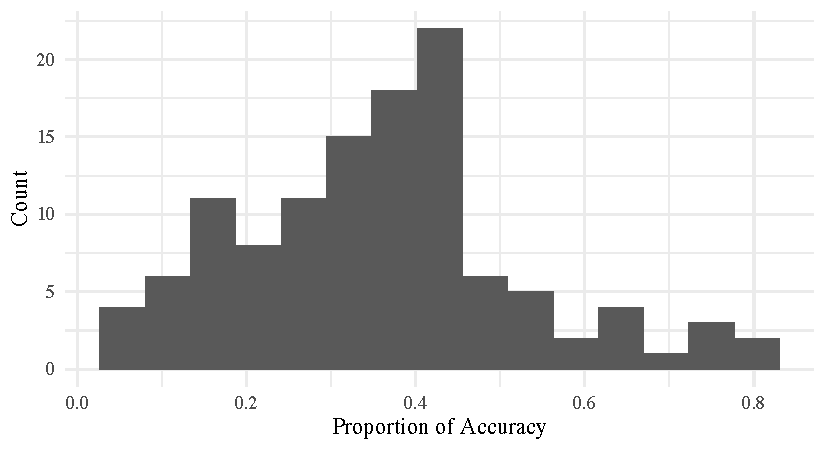
\includegraphics[width=\linewidth]{figure/exp1gFillHistogram-1} 

}

\caption[The accuracy histogram of grammatical fillers in Experiment 1]{The accuracy histogram of grammatical fillers in Experiment 1}\label{fig:exp1gFillHistogram}
\end{figure}

\end{knitrout}

Figure \ref{fig:exp1AvgResponse} shows the average proportions of acceptable responses as a function of sentence grammaticality, attractor number, and experiment. Since we were specifically interested in whether or not there would be a difference in acceptability due to a local ambiguity, we grouped the averages into two facets according to the grammaticality of the sentence. By doing so, we have the categorical experiment (presence of local ambiguity) in the x-axis, making comparison easier. Additionally, the line type shows the attractor number.  

\begin{knitrout}
\definecolor{shadecolor}{rgb}{0.969, 0.969, 0.969}\color{fgcolor}\begin{figure}[hbt!]

{\centering 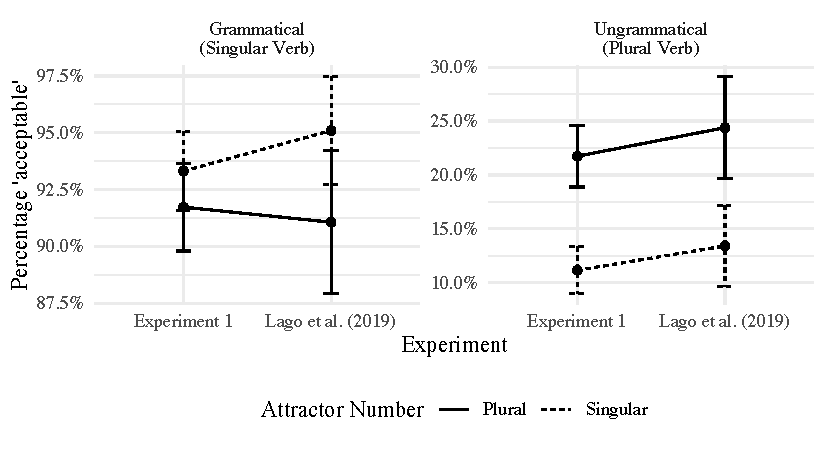
\includegraphics[width=\linewidth]{figure/exp1AvgResponse-1} 

}

\caption[The average percentage of acceptable responses according to the experimental conditions in our Experiment 1 and Lago et al.'s (2019) study]{The average percentage of acceptable responses according to the experimental conditions in our Experiment 1 and Lago et al.'s (2019) study}\label{fig:exp1AvgResponse}
\end{figure}

\end{knitrout}

With grammatical verbs, participants in both our experiment and \cites{LagoEtAl2019} study showed similar patterns. Accuracy rates were nearly equal (M = 0.92 and 0.93, SE = 0.01 and 0.01, for singular and plural attractors respectively) both in our experiment and in \cites{LagoEtAl2019} study (M = 0.91 and 0.95, SE = 0.02 and 0.01, for singular and plural attractors, respectively).

When we focus on our experimental results, we see that participants gave more acceptable responses in ungrammatical sentences with plural attractors (M = 0.22, SE = 0.01) compared to ungrammatical sentences with singular attractors (M = 0.11, SE = 0.01). The magnitude of the effect of plural attractor on ungrammatical sentences (0.11) were comparable to the \cites{LagoEtAl2019} results (0.11).

Figure \ref{fig:exp1RT} shows the average response times for correct responses as a function of sentence grammaticality, attractor number, and experiment. We have used the same layout as the one we used in \ref{fig:exp1AvgResponse}.

% \begin{knitrout}
% \definecolor{shadecolor}{rgb}{0.969, 0.969, 0.969}\color{fgcolor}\begin{figure}[hbt!]
% {\centering 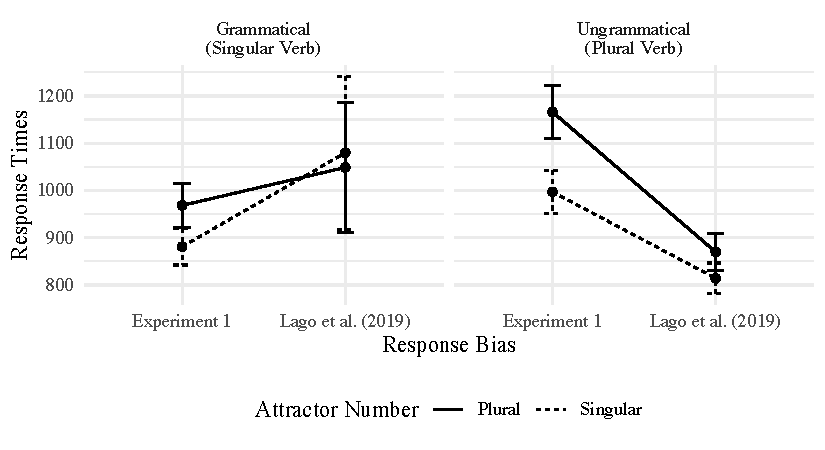
\includegraphics[width=\linewidth]{figure/exp1RT-1} 

% }

% \caption{The average response times according to the experimental conditions in our Experiment 1 and Lago et al.'s (2019) study}\label{fig:exp1RT}
% \end{figure}

% \end{knitrout}

\begin{figure}[hbt!]
{\centering 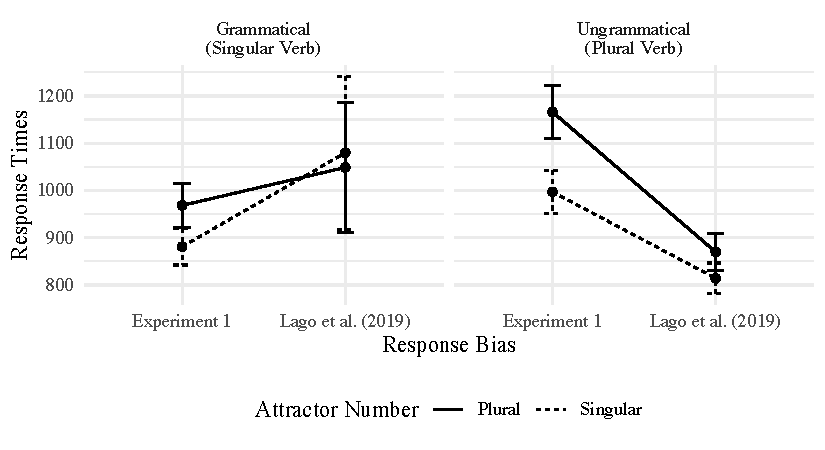
\includegraphics[width=\linewidth]{figure/exp1RT-1} 
}

\caption{The average response times according to the experimental conditions in our Experiment 1 and Lago et al.'s (2019) study}\label{fig:exp1RT}
\end{figure}


Our results suggest an overall slowdown in plural attractor conditions. This slowdown is evident in ungrammatical sentences. Participants gave faster responses when sentences include a singular attractor (M = 997.02, SE = 23.11) compared to a plural attractor (M = 1165.92, SE = 28.97). 


In Figure \ref{fig:exp1BayesPool}, we see the posterior probabilities for our Bayesian GLM model with a probit link, as well as ROPE borders and the probability of coefficients being smaller than $-0.1$. We used sentences from both our experiment and \cites{LagoEtAl2019} experiment. The negative main effect of ungrammaticality ($\hat{\beta}=-3.10;$ $CI=[-3.37; -2.86];$ $P(\beta>0.1)< .001$) indicated that participants were able to detect ungrammaticality both in our and \cites{LagoEtAl2019} experiment. Additionally, the positive interaction between the ungrammaticality and the plural attractor ($\hat{\beta}=0.76;$ $CI=[0.46; 1.04];$ $P(\beta>0.1)> .999$) meant that participants, on average, gave more \textit{yes} responses in ungrammatical sentences when there is a plural attractor. According to the posterior distribution of the coefficient trial no ($\hat{\beta}=0.03;$ $CI=[-0.05; 0.11];$ $P(\beta>0.1)   .04$), we infer that the order participants saw the experimental data did not affect the number of yes responses. Most importantly, a lack of evidence for the three-way interaction between the ambiguity, ungrammaticality, and the plural attractor ($\hat{\beta}=0.26;$ $CI=[-0.25; 0.76];$ $P(\beta>0.1)   .74$) suggested that the local ambiguity did not affect the grammaticality illusion. In other words, the magnitude of a plural attractor's effect in ungrammatical sentences was not contingent on the local ambiguity.

% \begin{knitrout}
% \definecolor{shadecolor}{rgb}{0.969, 0.969, 0.969}\color{fgcolor}\begin{figure}[hbt!]
% {\centering 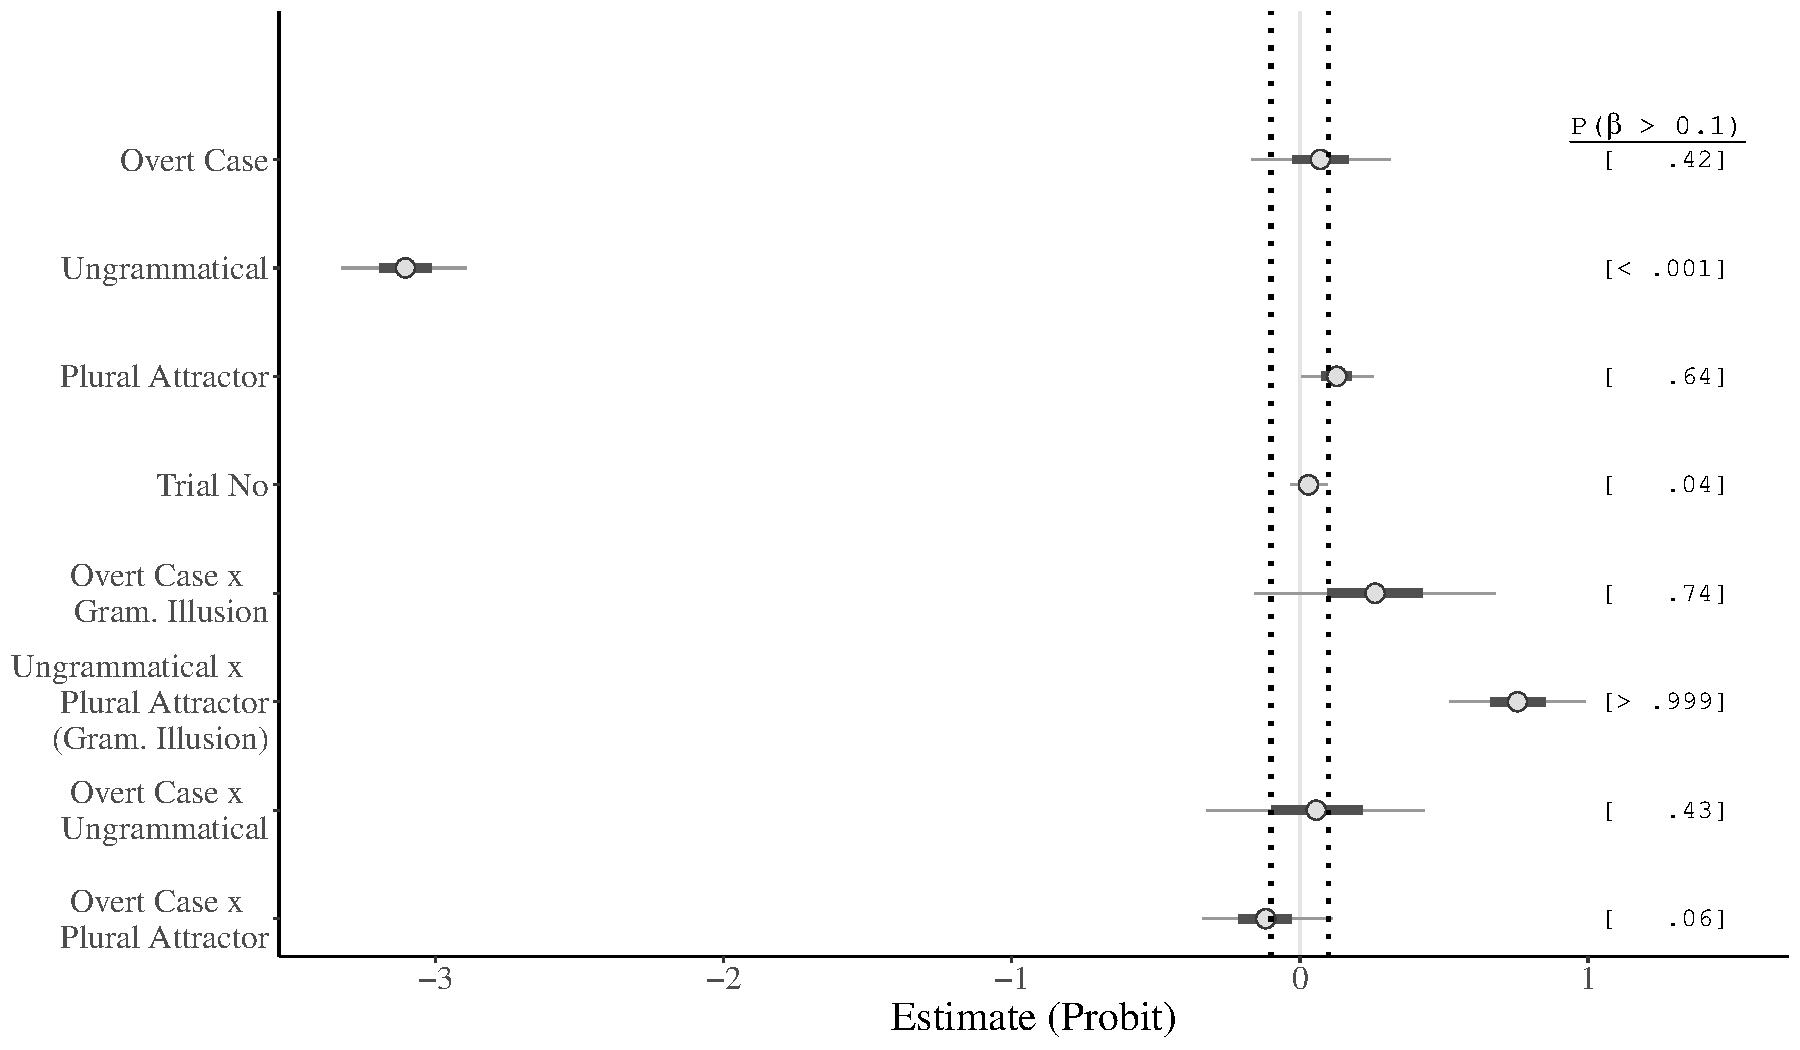
\includegraphics[width=\linewidth]{figure/exp1BayesPool-1} 
% }
% \caption{Estimates and 95\% credible intervals for the probit regression coefficients for the model of responses in our experiment and \citet{LagoEtAl2019}}\label{fig:exp1BayesPool}
% \end{figure}
% \end{knitrout}

\begin{figure}[hbt!]
{\centering 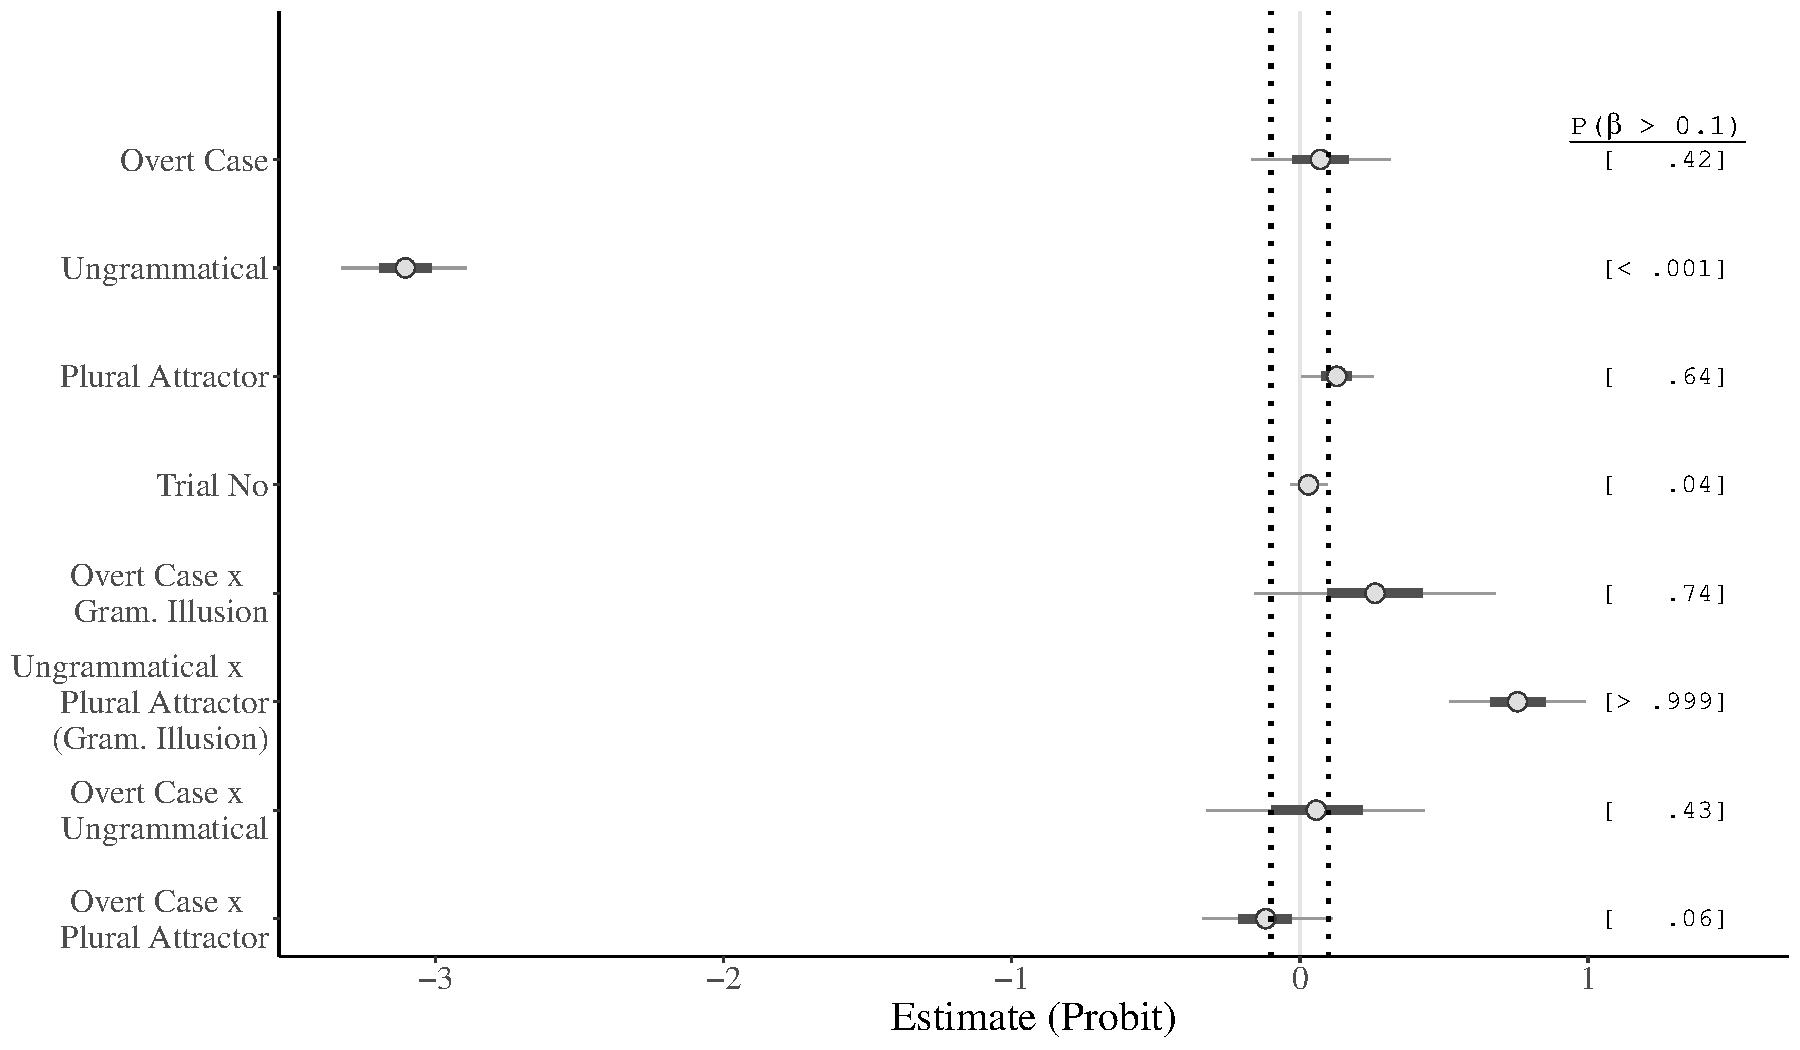
\includegraphics[width=\linewidth]{figure/exp1BayesPool-1} 
}
\caption[Estimates and 95\% credible intervals for the probit regression coefficients for the model of responses in our experiment and Lago et al. (2019)]{Estimates and 95\% credible intervals for the probit regression coefficients for the model of responses in our experiment and \citet{LagoEtAl2019}}\label{fig:exp1BayesPool}

\end{figure}

Figure \ref{fig:exp1BayesUngram} shows the estimates of a model based on only the ungrammatical sentences from both studies. The lack of evidence presented in \ref{fig:exp1BayesPool} is also supported in this model. Our second model showed no evidence for an interaction between the local ambiguity and the presence of a plural attractor ($\hat{\beta}=0.02;$ $CI=[-0.30; 0.34];$ $P(\beta>0.1)   .32$). Our second model also showed no main effect for the order of trials presented ($\hat{\beta}=-0.04;$ $CI=[-0.14; 0.07];$ $P(\beta>0.1)  .006$) and for the ambiguity ($\hat{\beta}=0.03;$ $CI=[-0.32; 0.38];$ $P(\beta>0.1)   .35$), meaning that independent of the presence of plural attractor local ambiguity did not affected the percentage of yes responses. Lastly, a more evidence for the plural attractor ($\hat{\beta}=0.48;$ $CI=[0.30; 0.67];$ $P(\beta>0.1)> .999$) were present in our second model compared to the first model. We infer from this difference that the ungrammatical sentences mainly drove the main effect of the plural attractor in the first model.


\begin{knitrout}
\definecolor{shadecolor}{rgb}{0.969, 0.969, 0.969}\color{fgcolor}\begin{figure}[hbt!]

{\centering 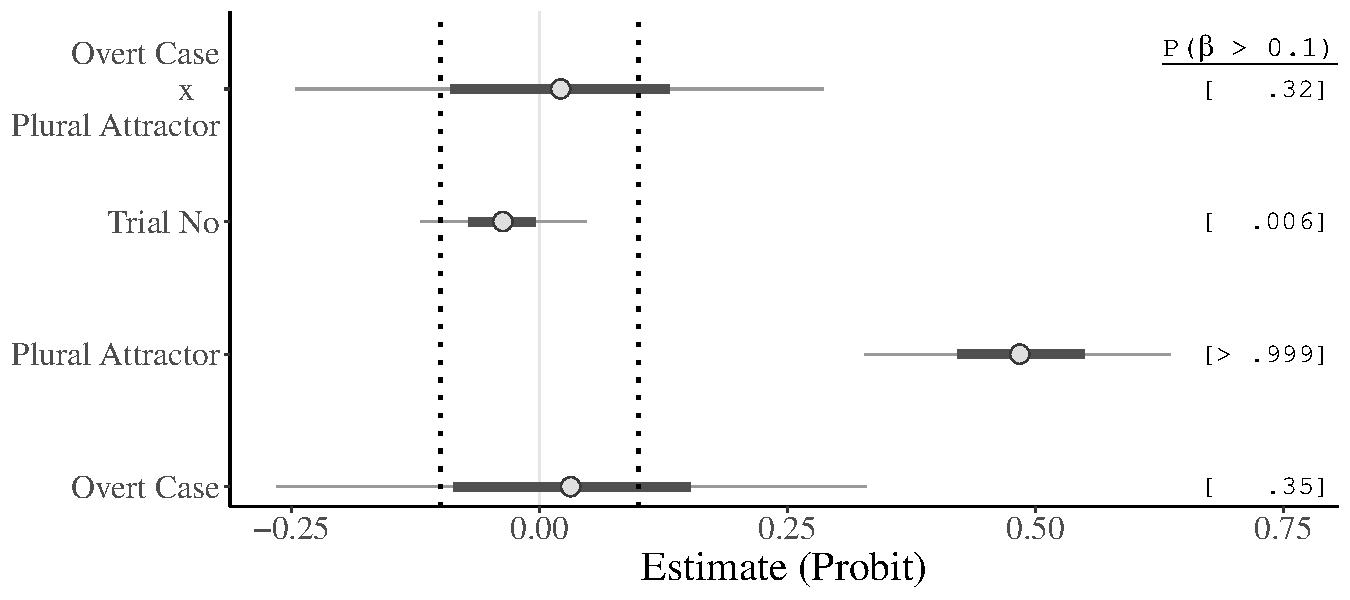
\includegraphics[width=\linewidth]{figure/exp1BayesUngram-1} 

}

\caption[Estimates and 95\% credible intervals for the probit regression coefficients for the model of responses to ungrammatical sentences in our experiment and Lago et al. (2019)]{Estimates and 95\% credible intervals for the probit regression coefficients for the model of responses to ungrammatical sentences in our experiment and \citet{LagoEtAl2019}}\label{fig:exp1BayesUngram}
\end{figure}
\end{knitrout}

\section{Discussion}

This chapter examined the alternative hypothesis that might explain the Turkish agreement attraction findings with genitive-possessive constructions. We hypothesized that the local ambiguity due to the syncretism between the possessive and the accusative case in \cites{LagoEtAl2019} items might be the main factor in their findings. We argued that participants might posit two different parses when they encounter \emph{NP-\Gen{} NP-i} strings. They would associate the head \emph{NP-i} with a non-subject case in one possible parse. This, in turn, reduces the association between the head \emph{NP-i} and the subjecthood. If that was the case and the previous findings were due to the lingering association between the noun \emph{NP-i} and the objecthood, then we expected not to find an agreement attraction effects in sentences where the case on the head \emph{NP-i} is unambiguous.

Our results suggested that participants accepted ungrammatical sentences with plural attractors more often than ungrammatical sentences with singular attractors even when the subject head is disambiguated. This finding is comparable to mainstream agreement attraction and \cites{LagoEtAl2019} findings. 

Additionally, our initial Bayesian model showed no interaction between the grammaticality illusion (the agreement attraction) and the local ambiguity. That is, manipulating the presence of the local ambiguity did not change the acceptability difference between the plural attractor-ungrammatical and the singular-attractor ungrammatical conditions. Our second model, which only included ungrammatical sentences, verified these findings: there was no interaction between the local ambiguity and the attractor number. Our model results suggested that the agreement attraction was not contingent on the local ambiguity and the head NP's reduced association with the subjecthood due to lingering effects of alternative parses. 

In light of our findings and \cites{LagoEtAl2019} findings, existing agreement attraction findings cannot be explained via our hypothesis based on the inhibitory effects of a possible parse where a subject head is parsed as a direct object. Additionally, we can say that local ambiguities stemming from the marking on the head noun do not give rise to additional grammaticality illusions. Unlike previous findings on the role of case syncretism in agreement attraction \citep{Slioussar2018}, our results suggested that participants did not utilize cues based on the form. This difference was because the syncretism in \citeand{Slioussar2018} was introduced in the attractor, whereas the syncretism in our study was related to the marking on the subject head. It seemed that when the manipulation done on the syntactically more prevalent elements, participants did utilize abstract linguistic cues. Thus, our results point towards an attraction account where the syntactic difference between the head and the attractor plays a significant role.
